\section{System Considerations}
If not explicitly mentioned, the system's settings are as follows:
\subsubsection*{Ensemble}
$N$ particles in a box of volume $V$ and temperature $T$ are considered.
The closed box is placed in an external heat bath, hence the total energy is not fixed and the probability $P_i$ for a given State $\ket{i}$ with Energy $E_i$ and $\beta \mathrel{\mathop:}= \frac{1}{kT}$ is given by
\begin{align}
	P_i = \frac{1}{Z}\exp\left(-\beta E_i\right)\text{, and }
	Z = \sum_k \exp\left(-\beta E_k\right).
\end{align}
Such an ensemble is called canonical or NVT.

\subsubsection*{Potential and Energy}
The particles are interacting via a normed Lennard-Jones Potential
\begin{align}
\label{LJPot}
	V_{ij} = 4\left(\frac{1}{r_{ij}^{12}} - \frac{1}{r_{ij}^6} + \frac{2^7 - 1}{2^{14}}\right),
\end{align}
such that $V_{ij}=0$, if $r_{ij} = 2\sqrt[6]2$.
The total energy $E_n$ of the system in a state $\ket{n}$ is given by the expression
\begin{align}
	E_n = \sum_i\sum_{j\neq i}V_{ij}.
\end{align}
\newpage
\subsubsection*{Periodic Boundary Conditions}
For both implementations, periodic boundary conditions (PBC) will be used, which imply two important consequences: \smallskip\\
First, when a particle reaches the border of the System, it is not reflected back, but transfered to the other side of the box.
A visualisation can be found in Fig.~\ref{Fig:PBCJump}.
\begin{figure}[h!]
\centering
\begin{minipage}[c]{\textwidth}
\begin{minipage}[c]{0.475\textwidth}
	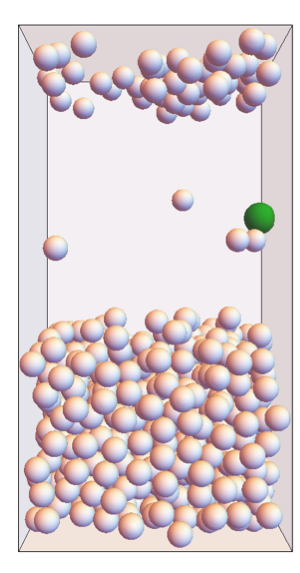
\includegraphics[width=\textwidth]{BoundaryJump.png}
\end{minipage}
\begin{minipage}[c]{0.475\textwidth}
	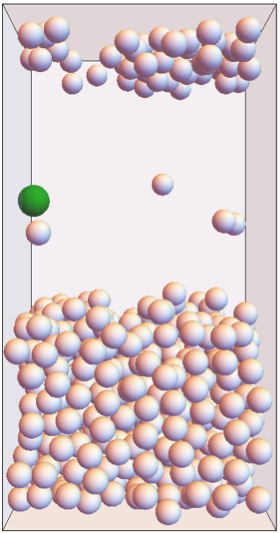
\includegraphics[width=\textwidth]{BoundaryJump2.png}
\end{minipage}
\end{minipage}
\caption[PBC: Jump Case]{A particle in a box with PBC jumps from one side to the other.}
\label{Fig:PBCJump}
\end{figure}\\
Second, particles can interact with images of other particles behind the border of the box. As a result, the distance vector between two particles is not unique.
\begin{figure}[h!]
\centering
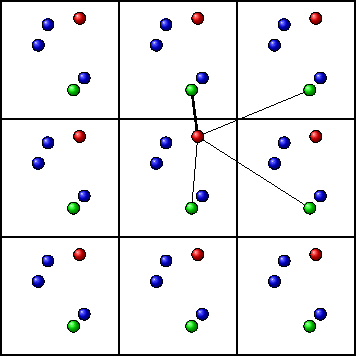
\includegraphics[width=0.8\textwidth]{Figures/tikz/MinimalDistance.pdf}
\caption[PBC: Interaction Case]{Box $S$ at the center represents the simulation box.
All other images A - H are induced products of PBC and do not exist in the simulation.
The crutial thing is the non unique distance between interacting particles as a result.}
\label{PBCinteraction}
\end{figure}
A particle neighter interacts with itself nor {\em all} of its images, hence the minimum image convention is applied.
This means a particle's contribution to the potential energy are interacitons with the {\em closest} images of all other particles.
In Fig.\ref{PBCinteraction}, the shortest distance is represented with a thick black line.





